%\documentclass[12pt,fleqn]{article}
%\usepackage{amsmath,epsfig,epsf,psfrag,natbib,lineno,hyperref,setspace}


\documentclass[aoas,preprint]{imsart}

\RequirePackage[OT1]{fontenc}
\RequirePackage{amsthm,amsmath,lineno,epsfig,epsf,psfrag}
\RequirePackage[]{natbib}
\RequirePackage[colorlinks,citecolor=blue,urlcolor=blue]{hyperref}
\usepackage[nolists,nomarkers]{endfloat}

\startlocaldefs
\numberwithin{equation}{section}
\theoremstyle{plain}
\newtheorem{thm}{Theorem}[section]
\endlocaldefs

\begin{document}

\def\VAR{{\rm Var}\,}
\def\COV{{\rm Cov}\,}
\def\Prob{{\rm P}\,}
\def\bfX{\textbf{X}}
\def\bfY{\textbf{Y}}
\def\bfZ{\textbf{Z}}
\def\bfD{\textbf{D}}
\def\bfz{\textbf{z}}
\def\bfy{\textbf{y}}
\def\bfd{\textbf{d}}
\def\bfx{\textbf{x}}
\def\bfbeta{\boldsymbol{\beta}}
\def\bfdelta{\boldsymbol{\delta}}
\def\bfeta{\boldsymbol{\eta}}
\def\bfphi{\pmb{\phi}}
\def\bftheta{\pmb{\theta}}
\def\bfpsi{\pmb{\psi}}
\def\bfPsi{\pmb{\Psi}}
\def\bfpi{\pmb{\pi}}
\def\bfp{{\bf p}}
\def\bfGamma{\pmb{\Gamma}}



\begin{frontmatter}
\title{Simultaneous modelling of movement, measurement error, and observer dependence in mark-recapture distance sampling: an application to Arctic bird surveys}
\runtitle{Distance sampling with movement}

\begin{aug}
\author{\fnms{Paul B.} \snm{Conn}\thanksref{t1}\ead[label=e1]{paul.conn@noaa.gov}}
\and
\author{\fnms{Ray T.} \snm{Alisauskas}\thanksref{t2}\ead[label=e2]{ray.alisauskas@canada.ca}}

\affiliation{Marine Mammal Laboratory, Alaska Fisheries Science Center, National Marine Fisheries Service, NOAA\thanksmark{t1} and Wildlife Research Division, Environment and Climate Change Canada\thanksmark{t2}}

\address{7600 Sand Point Way NE\\
Seattle, WA 98115 USA \\
\printead{e1} }
%\phantom{E-mail:\ }\printead*{e1}}

\address{Prairie and Northern Wildlife Research Centre\\
115 Perimeter Rd.\\
Saskatoon, SK S7N 0X4 CANADA\\
\printead{e2} }
%\printead{u1}}
\end{aug}

\begin{abstract}
Mark-recapture distance sampling is a promising method for surveying bird populations from aircraft in open landscapes. However, commonly available distance sampling estimators require that distances to target animals are made without error and that animals are stationary while sampling is being conducted.  Motivated by a recent bird survey where these requirements were routinely violated, we describe a marginal likelihood framework for estimating abundance from double-observer data that can accommodate movement and measurement error when observations are made consecutively (as with front and rear observers), when animals are uniformly distributed during detection by the first observer, and when detections consist of both moving and stationary animals.  Assuming that all animals are subject to measurement error and that some animals can move between detections, we integrate over unknown animal locations to construct a marginal likelihood for detection, movement, and measurement error parameters. Estimates of animal abundance are then obtained using a modified Horvitz-Thompson-like estimator.  In addition, unmodelled heterogeneity in detection probability can be accommodated through observer dependence parameters.  Using simulation, we show that our approach yields low bias compared to approaches that ignore movement and/or measurement error, including in cases where there is considerable detection heterogeneity.  Applying our approach to data from a double-observer waterfowl helicopter survey in northern Canada, we are able to estimate bird density accounting for movement and measurement error and corrected for observer heterogeneity.  Our approach appears promising for generating unbiased estimates of bird abundance necessary for reliable conservation and management.
\end{abstract}

%\begin{keyword}[class=MSC]
%\kwd[Primary ]{60K35}
%\kwd{60K35}
%\kwd[; secondary ]{60K35}
%\end{keyword}

\begin{keyword}
\kwd{aerial survey}
\kwd{double-observer}
\kwd{mark-recapture distance sampling}
\kwd{measurement error}
\kwd{movement}
\kwd{point independence}
\end{keyword}

\end{frontmatter}

\linenumbers






\section{Introduction}

Distance sampling surveys \citep{BurnhamEtAl1980,BucklandEtAl2001} are often used to estimate the abundance of wildlife populations.  Such surveys were historically conducted by a single observer who followed a transect line and recorded the perpendicular distance to each detected animal group.  Assuming 100\% detection on the transect line, investigators can fit models to estimate abundance over the surveyed area while accounting for detection probabilities that decline with distance from the transect line.

When surveys are conducted from the air, double-observer surveys have major advantages over single-observer surveys.  For instance, one can use records of detection/non-detection to relax the assumption of perfect detection on the transect line \citep{BorchersEtAl1998}.  Analysis of double-observer distance data is now canonically referred to as ``mark-recapture distance sampling" \citep[MRDS; ][]{LaakeBorchers2004} because there is a detection history (i.e. binary detection/nondetection records for each observer) in addition to recorded distances.

Despite the potential usefulness of MRDS methods for estimating abundance, published methods often assume that animals do not move between detections of observers, and that distances are recorded without error.  These assumptions are problematic for some species and sampling situations, such as aerial surveys of birds where individuals may exhibit responsive movement away from aircraft.
Several authors have investigated consequences and corrections for movement in distance sampling applications.  For instance, \citet{GlennieEtAl2015} showed that movement could cause considerable bias (typically positive) in distance-based abundance estimators, but did not attempt to develop methods to adjust for such bias. \citet{HibyLovell1998} developed a likelihood framework to estimate abundance when movement is random (i.e. nonresponsive to the survey platform) and occurs between successive observations; however, their approach does not account for responsive movement away from the survey platform.

Likewise, \citet{BorchersEtAl2010} showed that measurement errors could cause substantial (usually positive) bias in distance sampling abundance estimators. A number of authors have proposed models that account for measurement error in specific distance sampling applications \citep[see e.g.][and references therein]{SchwederEtAl1999,BorchersEtAl2010}.

Several observer configurations are possible within an MRDS estimation framework \citep{BurtEtAl2014} and have important implications for bias control when animals move in response to a survey platform (i.e. ``responsive" movement).  In an ``independent" configuration, observers detect animals independently of one another.  Under this configuration it is possible to try to account for heterogeneity in detection probabilities (e.g. visual distinctiveness of different animal groups) by modelling lack of fit between the distribution of observed distances and estimated detection probabilities as a function of distance \citep{LaakeBorchers2004,BorchersEtAl2006,BucklandEtAl2010}.  The ability to account for such heterogeneity is important because abundance estimators are negatively biased otherwise. Alternatively, in a ``trial" configuration \citep{BucklandTurnock1992}, one observer searches ahead, while another searches closer to the survey platform.  Under this configuration, detections by the first observer are used as trials for the second observer.  The trial configuration is useful for reducing bias associated with responsive movement of animals (which often positively biases abundance estimators), but one can no longer model heterogeneity in detection probability \citep{BurtEtAl2014}.

In this paper, we develop an integrated likelihood framework to account for movement and measurement error using an independent observer MRDS configuration. Our development is motivated by aerial surveys of birds, where the goal is to unbiasedly estimate the species densities needed for effective monitoring and conservation decisions. As such, we address movement between the time that two observers (e.g. front and rear seat observers on the same side of the aircraft) are able to make detections.  Our objective is to account for the biasing effects of measurement error and responsive movement while also being able to model individual heterogeneity through an observer dependence specification.  The remainder of this article is structured as follows.  First, we describe a motivating data set, in which distances, detection histories, and individual covariates are summarized from a double-observer aerial survey in northern Canada.  Second, we describe a maximum marginal likelihood (MML) framework for analyzing these data.  Under this framework, true animal locations are treated as latent variables.  Next, we illustrate our method by analyzing the waterfowl data set and examine estimator performance with two simulation studies.  We conclude with a short discussion on our proposed modeling framework, future research needs, and some specific suggestions related to bird survey applications.


\section{Waterfowl data}

In June of 2014, biologists conducted a pilot double-observer helicopter (BELL 206L on floats) survey of Arctic bird species in the Queen Maud Gulf Migratory Bird Sanctuary (Nunavut, Canada; Fig. \ref{fig:map}). The total length of survey tracks was 947.8km.  Birds surveyed were predominantly waterfowl, but also included cranes and ptarmigan; we refer to them collectively as waterfowl for the remainder of the paper. The original intent of the survey was to investigate the potential of MRDS methods for surveying Arctic waterfowl, and to compare them to other commonly used waterfowl survey methods such as those that use double observers but don't record distance \citep[e.g.][]{KoneffEtAl2008}.  It was thus conducted opportunistically, lacking a sampling frame needed for extrapolation to larger areas.
The survey is described in greater detail elsewhere \citep{AlisauskasConn2017}, but we briefly provide information relevant to the analysis conducted later in this paper.

During the survey, two observers, one behind the other, on the same (left) side of the helicopter independently detected and recorded the perpendicular distance from the transect line to each bird group they observed.  Distances were binned into 6 classes: 0-40m, 40-80m, 80-120m, 120-160m, 160-200m, and 200m+ (note that observations in the final bin are not used in subsequent analysis).  They also recorded species, the number of waterfowl in each detected group (``group"), and a binary indicator for whether the waterfowl group was flapping their wings (``moving").  These data were previously analyzed by \citet{AlisauskasConn2017}, who used standard MRDS methods that ignored movement and measurement error in their analysis.  Their analysis suggested that moving birds were more detectable than stationary ones, that detection probability increased with group size, and that the front seat observer had higher detection probability than the rear seat observer.  They also estimated similar species effects on detection for 7 of the 9 species analyzed; here, we analyze detections of these 7 species (Canada goose, king eider, long-tailed duck, northern pintail, rock ptarmigan, sandhill crane, and white-fronted goose), within the same model to illustrate modeling concepts.  This protocol led to a total of 964 unique waterfowl group detections; 359 were detected by both observers, 348 by the front observer only, and 257 by the back observer only.  Note that the back seat observer's view of the first distance bin nearest the transect line was partially obstructed by the left helicopter float.  A plot of observed distance deviations suggested asymmetrical responsive movement (away) from the aircraft for nonstationary animal groups.  There were also some minor distance discrepancies for animal groups that were not moving, suggesting measurement error (Fig. \ref{fig:dist_hists}).

The observed distribution of distances is problematic in the sense that it explicitly contradicts the standard MRDS modeling assumption that animals do not move between successive observations. Further, they make individual heterogeneity difficult to diagnose because the patterns in distance data that are indicative of heterogeneity can be obscured by patterns due to distance. This leads to some natural questions: first, what degree of bias might we expect in estimates of animal abundance when classical MRDS models are applied to data like ours?  Second, is it possible to mitigate bias in estimates of abundance by explicitly modelling the movement and measurement error processes?  We now attempt to develop such a framework before conducting some small simulation studies to investigate bias of our proposed procedure relative to classical approaches that ignore movement and measurement error.

\section{Model development}

Distance sampling surveys seek to estimate the abundance, $N$, of an animal population in a given survey region. However, only a fraction $p_c$ of the survey region is covered by transects, so it is customary to focus on estimation of animal abundance in the ``covered region," $N_c$, and then to use design-based procedures to expand this estimate to the full study area (e.g. $\hat{N}=N_c/p_c$).  In the present paper, we focus on estimation of $N_c$, with the understanding that such estimates can easily be expanded to a larger study area if desired \citep[e.g.][]{BucklandEtAl2004}.  For notational ease, we shall use $N$ to represent $N_c$ for the remainder of the paper.

Consider a double-observer MRDS survey where each observer records binned distances to detected animal groups, independently of the other observer, and a total of $n$ animal groups are encountered by at least one observer (see Table \ref{tab:notation} for a complete list of notation).  We develop a two-stage approach for estimating abundance in the surveyed area from such data.  In the first step, a MML framework is used to simultaneously estimate parameters of detection, movement, and measurement error processes.  In the second, a Horvitz-Thompson-like estimator is used to estimate abundance conditioned on parameter estimates from step 1.

In MRDS surveys with binned distances, observers record animals as occurring in one of $n_\mathcal{S}$ perpendicular distance bins, $\mathcal{S} = \mathcal{S}_1,\mathcal{S}_2,\hdots,\mathcal{S}_{n_\mathcal{S}}$.  Detection probability typically decreases with distance from the transect line, and the maximum distance bin is often set such that animals farther away can be ignored without greatly affecting precision of abundance estimates.  Movement and measurement error introduce complications: in addition to such errors among elements of $\mathcal{S}$, animals can potentially move into or out of $\mathcal{S}$, and animals outside of $\mathcal{S}$ can be detected in $\mathcal{S}$.  For these reasons, the models we develop rely on augmenting $\mathcal{S}$ with additional distance bins to allow for movement and measurement error (Fig. \ref{fig:aug_bins}).  Call this augmented set $\mathcal{Z}$.

Let $y_{io}$ be a binary indicator for whether or not the $i$th animal group was detected by observer $o$.  Similarly, let $d_{io}$ denote the distance bin recorded by observer $o$ for animal group $i$ (note $d_{io}$ is only defined when $y_{io}=1$). We assume that distances are only recorded within the truncation range of the transect, so $y_{io}=0$ whenever an animal group is perceived as having $d_{io} \notin \mathcal{S}$.  Letting bold upper case symbols denote matrices (e.g. ${\bf Y}$ is a ($2 \times n$) matrix of all detection/nondetections),  we seek to define a joint density function $[{\bf Y},{\bf D}|\boldsymbol{\theta},{\bf X}]$, where $\boldsymbol{\theta}= \{ \boldsymbol{\beta,\phi,\varphi} \}$ are parameters describing probabilities of detection, movement, and measurement error, respectively, and ${\bf X}$ includes individual covariates collected for each animal group that can be used to explain variation in detection probabilities.  Note that here and throughout the paper, we use the bracket notation(e.g.  $[\bfY|\bfX]$) to denote the conditional distribution of $\bfY$ given $\bfX$; we treat responses (e.g. $\bfY$, $\bfD$) as random variables under this construction even though it is not explicitly written.

\subsection{Likelihood}

To construct an appropriate likelihood for statistical inference, we start with the general framework proposed by \citet{BorchersEtAl2015} for spatial mark-recapture and distance sampling surveys.  Conditioning on detection, \citet{BorchersEtAl2015} suggested that the joint distribution of animal locations and detections could be written as a product of (1) a joint probability density function (pdf) for the latent locations of animals, and (2) a joint probability mass function (pmf) for the encounter histories conditional on location.  We expand upon this framework to allow movement to affect the distribution of animal locations and to incorporate a measurement error mechanism.

Letting $z_{io}$ denote the true location (latent distance bin) of animal group $i$ when it enters the field of view of observer $o$, we write the joint probability mass function of observed data as a product of
\begin{enumerate}
   \item $[{\bf Z}|\boldsymbol{\theta}]$, a bivariate probability mass function for the distribution of true animal locations, given detection by at least one observer; and
   \item $[{\bf Y},{\bf D}|{\bf Z},\boldsymbol{\theta},{\bf X}]$, a model for binary detections and observed distances given true unobserved locations and individual detection covariates.
\end{enumerate}
If we knew the true locations of observed animals, we could simply base inference on the likelihood $\mathcal{L}(\boldsymbol{\theta};{\bf Z},{\bf D},{\bf Y},{\bf X})$ with corresponding joint density function
\begin{eqnarray*}
  [{\bf Z},{\bf D},{\bf Y}|\boldsymbol{\theta},{\bf X}] & = & [{\bf Y},{\bf D}|{\bf Z},\boldsymbol{\theta},{\bf X}][{\bf Z}|\boldsymbol{\theta}].
\end{eqnarray*}
However, we do not know the true animal locations so instead integrate (sum) over an augmented set of distance bins $\mathcal{Z}$ that could plausibly have resulted in a detection (see \textit{Distribution of animal locations} for more discussion of bin augmentation).
As such, we write the marginal likelihood of detection, movement, and measurement error parameters as $\mathcal{L}(\boldsymbol{\theta};{\bf D},{\bf Y},{\bf X})$, which corresponds to the joint density
\begin{equation}
  [{\bf Y},{\bf D}|\boldsymbol{\theta},{\bf X}] = \prod_i \left( \sum_{z_{i1} \in \mathcal{Z}} \sum_{z_{i2} \in \mathcal{Z}} [y_{i1},y_{i2}, d_{i1}, d_{i2}|z_{i1} , z_{i2}, \boldsymbol{\theta} , {\bf x}_i][z_{i1},z_{i2}  |\boldsymbol{\theta}]
   \right).
  \label{eq:lik}
\end{equation}
Recall that $z_{i o}$ is the true distance bin associated with animal group $i$ when it passes observer $o$.  Similarly, $y_{io}$ gives detection/nondetection, and $d_{io}$ gives observed distance values (which are missing whenever $y_{io}=0$), and $\bfx_i$ is a vector of covariates for individual $i$.  We now describe each of the likelihood components in further detail.  We shall make an attempt to redefine various quantities when needed; we also provide parameter definitions in Table \ref{tab:notation}.

\subsubsection{Distribution of animal group locations}

The first component of the joint density (Eqn. \ref{eq:lik}) is the joint mass function for the locations of group $i$, $[z_{i1},z_{i2}|\boldsymbol{\theta}]$, given detection by at least one observer.  We write this distribution as a function of (i) an initial state distribution, $[z_{i1}]$; (ii) a movement kernel, $[z_{i2}|z_{i1},\boldsymbol{\phi}]$; and (iii) detection probability by at least one observer, $p_i^*(z_{i1},z_{i2})$.  Specifically, we set
\begin{eqnarray}
[z_{i 1},z_{i 2} |\boldsymbol{\theta}] & \propto & [z_{i1}][z_{i2}|z_{i1},\boldsymbol{\phi}]p_i^*(z_{i1},z_{i2}),
\label{eq:z}
\end{eqnarray}
where the `$\propto$' sign indicates normalization such that $[z_{i 1},z_{i 2} |\boldsymbol{\theta}]$ sums to 1.0.
We explicitly include the thinning probability $p_i^*(z_{i1},z_{i2})$ in this component since observations in the data set are conditional on detection, and thus the position of observed animals are more likely to be close to the transect line than far away from it.

We make the common distance sampling assumption \citep[cf.][]{BucklandEtAl2001} that perpendicular distances of animals groups from the transect line are uniformly distributed when entering the field of view of the first observer.  This seems reasonable in applications where the first observer has a field of view facing forward, and when the survey platform moves fast relative to the speed of focal taxa (as in our waterfowl example; see Discussion for further consideration of this assumption). Letting $\pi_j$ denote the proportional diameter of distance bin $j$ (i.e. $\pi_j = a_j / \sum_k a_k$ where $a_j$ is the diameter of of distance bin $j$), the (continuous) uniform distance assumption translates into the following model for the latent distance bin of animal group $i$ when encountered by the first observer:
\begin{eqnarray*}
  z_{i1} & \sim & \text{Categorical}(\pi_1,\pi_2,\hdots,\pi_{n_{\mathcal{Z}}}),
\end{eqnarray*}
where it is understood that ``Categorical" denotes a multinomial distribution with index 1, and $n_{\mathcal{Z}}$ is the number of latent distance bins.

Next, the bivariate movement pmf $[z_{i2}|z_{i1},\boldsymbol{\phi}]$ describes the location of animal group $i$ when it enters the field of view of observer 2 as a function of the location when it was in the field of view of observer 1.  We model this as another categorical distribution:
\begin{eqnarray}
  [z_{i2}|z_{i1},\boldsymbol{\phi}] & = & \text{Categorical} \left( \psi(z_{i1},1),\psi(z_{i1},2),\hdots,\psi(z_{i1},n_\mathcal{Z}) \right).
  \label{eqn:move}
\end{eqnarray}
For applications in this paper, we parameterize the movement transition probabilities $\boldsymbol{\psi}$ using asymmetric kernels $k$ (e.g. Fig \ref{fig:kernel}).  Using an asymmetric kernel can allow movement rates to vary based on the direction of animal movement.  In particular, responsive movement away from the transect line may be more likely than movement towards the transect line. In particular, we set
\begin{linenomath*}
\begin{equation}
  \psi(z_{i1},z_{i2}) \propto k(z_{i1},z_{i2}|\boldsymbol{\phi}) \text{, where}
  \label{eq:psi}
\end{equation}
\begin{equation}
  k(z_{i1},z_{i2}|\boldsymbol{\phi}) = \left\{ \begin{array}{rl}
                                    f(\delta_{i2}|\mu=\delta_{i1},\sigma=\phi_1) & z_{i2}<z_{i1}, m_i = 1 \\
                                    f(\delta_{i2}|\mu=\delta_{i1},\sigma=\phi_2) & z_{i2} \ge z_{i1}, m_i = 1  \\
                                    1.0 & z_{i2}=z_{i1}, m_i=0 \\
                                    0.0 & z_{i2} \ne z_{i1}, m_i=0.
                                    \end{array} \right.
  \label{eq:g}
\end{equation}
\end{linenomath*}
Here, $f()$ gives a probability density function; in our examples, we consider Laplace (double exponential) and Gaussian distributions as choices for $f()$. Note that $\delta_{io}$ gives the perpendicular distance from the transect line to the midpoint of distance bin $z_{io}$, and that $\phi_1$ and $\phi_2$ are unknown scale parameters of the movement kernels.  Also note that we assume that stationary animals (i.e. with $m_i=0$) do not change distance bins.

Finally, the thinning probability
$p_i^*(z_{i1},z_{i2})$ is the probability of being detected by at least one observer for an animal that is in distance bin $z_{i1}$ at time 1 and $z_{i2}$ at time 2. It is a function of both detection probability and measurement error parameters:
\begin{eqnarray*}
  \label{eq:pstar}
  p_i^*(z_{i1},z_{i2}) & = &
  1 - [1- p_{i1}(z_{i1}) \omega(z_{i1},\mathcal{S})][1-p_{i2}(z_{i2})\omega(z_{i2},\mathcal{S})],
\end{eqnarray*}
where $p_{io}(z_{io})$ is the probability of observer $o$ detecting group $i$ when it is at distance $z_{io}$, and $\omega(z_{io},\mathcal{S})$ is the probability that the observer perceives the group to be within the truncation range ($\mathcal{S}$) of the transect.  This expression is slightly different than typically encountered in MRDS models, as one must account for two ways of getting a 0 in a capture history: an observer can either miss the animal group or detect the group but determine it to be outside the truncation range of the transect (i.e. $\notin \mathcal{S}$).  To account for the latter possibility, we make use of the measurement error probabilities $\omega(z,d)$, which can be parameterized in terms of a measurement error kernel similarly to $\boldsymbol{\psi}$ (see Eqs. \ref{eq:psi}-\ref{eq:g}). Given a true distance bin $z$, we then compute $\omega(z,\mathcal{S})=\sum_{d \in \mathcal{S}} \omega(z,d)$. In applications in the paper, we consider use of symmetric measurement error kernels (Gaussian or Laplace) with a single scale parameter, $\varphi$.

In order to impart meaningful variation in detection probability, it is useful to express $p_{io}(z_{io})$ in a regression framework on a logit-linear scale, such that
\begin{eqnarray}
  \textrm{logit}({\bf p}) & = & {\bf X} \boldsymbol{\beta}.
  \label{eq:p}
\end{eqnarray}
where ${\bf X}$ is a design matrix and $\boldsymbol{\beta}$ is a vector of regression parameters.
Note that we shall often include $z_{io}$ (a latent quantity) within \textbf{X}; thus  the design matrix ${\bf X}$ will not be fixed as is customary in regression applications.  For example, suppose we desire a model where detection probability is a function of distance, squared distance, observer, and group size ($g_i$).  We could then formulate Eq. \ref{eq:p} such that
\begin{eqnarray}
  \left(
  \begin{array}{c}
    \textrm{logit}(p_{11}) \\
    \textrm{logit}(p_{12}) \\
    \textrm{logit}(p_{21}) \\
    \textrm{logit}(p_{22}) \\
    \vdots \\
    \textrm{logit}(p_{n1}) \\
    \textrm{logit}(p_{n2})
  \end{array}
  \right)
    & = &
  \left[
  \begin{array}{ccccc}
    1 & z_{11} & z_{11}^2 & 0 & g_1 \\
    1 & z_{12} & z_{12}^2 & 1 & g_1 \\
    1 & z_{21} & z_{21}^2 & 0 & g_2 \\
    1 & z_{22} & z_{22}^2 & 1 & g_2 \\
    \vdots & \vdots & \vdots & \vdots & \vdots \\
    1 & z_{n1} & z_{n1}^2 & 0 & g_n \\
    1 & z_{n2} & z_{n2}^2 & 1 & g_n
  \end{array}
  \right] \times
      \left[
  \begin{array}{c}
    \beta_0 \\
    \beta_1 \\
    \beta_2 \\
    \beta_3 \\
    \beta_4
  \end{array}
  \right].
  \label{eq:reg_ex}
\end{eqnarray}
Note that in the case of irregularly shaped bins, we would likely want to replace $z_{io}$ in Eq. \ref{eq:reg_ex} with distance bin midpoints.

\subsubsection{Likelihood of observed detections}

The next component of the joint density function is $[{ y}_{i1},{ y}_{i2},{ d}_{i 1},{ d}_{i 2}|{ z}_{i 1},{ z}_{i 2}, \boldsymbol{\theta} , {\bf x}_i]$, the probability of realizing different random variables for detection ($y_{i1}$ and $y_{i2}$) and associated  distance bin values ($d_{i1}$ and $d_{i2}$) for animal group $i$ conditional on true location.  Conditional on detection by at least one observer, there are three possible types of encounter histories: $h_i = `11'$ (encountered by both observers), $h_i = `10'$ (encountered by the first observer and not the second), and $h_i = `01'$ (encountered by the second observer but not the first).  For `11' histories, there are $n_\mathcal{S}^2$ combinations of possible recorded distance bins; for `10' histories, there are $n_\mathcal{S}$ distance bins possible for observer 1; for `01' histories, there are $n_\mathcal{S}$ distance bins possible for observer 2.  Thus, we can view $[{ y}_{i1},{ y}_{i2},{ d}_{i 1},{ d}_{i 2}|{ z}_{i 1} { z}_{i 2}, \boldsymbol{\theta} , {\bf x}_i]$ as a multinomial distribution with index 1 and $n_\mathcal{S}^2 + 2 n_\mathcal{S}$ possible outcomes. The likelihood contribution, $L_i$, for a particular animal group $i$ can thus be written as $L_i = (p_i^*(z_{i1},z_{i2}))^{-1} Pr(h_i)$, where the probability of observing each type of history is:
\begin{eqnarray*}
   Pr(h_i = `11') & = &  p_{i1}(z_{i1}) \omega(z_{i1},d_{i1}) p_{i2}(z_{i2}) \omega(z_{i2},d_{i2}), \\
   Pr(h_i = `10') & = & p_{i1}(z_{i1})\omega(z_{i1},d_{i1}) \left[
    p_{i2}(z_{i2})(1-\omega(z_{i2},\mathcal{S}))+(1-p_{i2}(z_{i2})) \right] \text{, and} \\
   Pr(h_i = `01') & = & p_{i2}(z_{i2})\omega(z_{i2},d_{i2}) \left[
    p_{i1}(z_{i1})(1-\omega(z_{i1},\mathcal{S}))+(1-p_{i1}(z_{i1})) \right].
\end{eqnarray*}
For a review of notation, see Table \ref{tab:notation}.

\subsection{Horvitz-Thompson-like abundance estimator}

Minimizing the negative log-likelihood associated with Eqn. \ref{eq:lik} provides marginal maximum likelihood estimates for detection, movement, and measurement error parameters, but does not provide a direct estimate of animal abundance, $N$.  We developed a Horvitz-Thompson-like procedure for $N$, as is common in distance sampling literature \citep[e.g.][]{BucklandEtAl2004}.  This is especially useful when coping with detection probabilities that vary as a function of individual detection covariates.  For instance, in standard MRDS applications, one might estimate abundance as
\begin{eqnarray*}
  \hat{N} & = & \sum_{i=1}^n \dfrac{g_i}{p_i^*},
\end{eqnarray*}
where $n$ is the number of animals detected, $g_i$ is the number of animals in group $i$, and $p_i^*$ is the probability of detection by at least one observer.
However, direct application of this estimator is clearly inappropriate under movement and measurement error, as it can potentially include animals outside of the surveyed area, or include animals that move into the surveyed area; thus, further development is needed.

We construct a Horvitz-Thompson-like estimator for abundance in the surveyed region $\mathcal{S}$ when animals enter the field of view of observer 1 (i.e. before any movement is assumed to occur) as follows:
\begin{eqnarray}
  \hat{N}|\hat{\boldsymbol{\theta}} & = & \sum_i \sum_{z_{i1} \in \mathcal{S}} \sum_{z_{i2} \in \mathcal{Z}} \frac{g_i \times [{z}_{i1},{z}_{i2} | \hat{\boldsymbol{\theta}}]}{p_i^*(z_{i1},z_{i2})}.
  \label{eq:ht}
\end{eqnarray}
This formulation integrates over the latent position of animal groups as they pass observers 1 and 2 (i.e. $z_{i1}$ and $z_{i2}$) with the restriction that they must be within the truncation range of the transect (i.e. $\in \mathcal{S}$) when they pass observer 1. The quantity $[{z}_{i1},{z}_{i2} | \hat{\boldsymbol{\theta}}]$ gives the discrete probability mass function for the true locations of detected animals evaluated at the MLEs.

As suggested by a reviewer, dependence on $p_i^*$ in the denominator of Eq. \ref{eq:ht} may lead to instability of the estimator if $p_i^*$ is low.  In distance sampling applications, it is thus common to replace $p_i^*$ with an expectation over $i$, $E(p^*)$ \citep[][Eq. 6.11]{LaakeBorchers2004}.
We leave examination of such a procedure to future research.

To compute variance, we adapt the approximation given independently by \citet{Huggins1989,Huggins1990} and \citet{Alho1990} and subsequently used by other authors in distance sampling applications \citep[e.g.][]{BorchersEtAl2006}.
This approach uses the law of total variance to write variance as a function of i) the variance associated with the number of animals encountered, and ii) variance associated with uncertainty in estimated parameters.  Specifically, our approximation is
\begin{eqnarray*}
  \hat{\text{Var}}(\hat{N}) & = & \sum_i \frac{(1-\tilde{p}_i)g_i}{\tilde{p}^2}+\hat{\textbf{D}}^\prime \hat{\boldsymbol{\Sigma}}\hat{\textbf{D}}, \text{ where} \\
  \tilde{p}_i & = & \sum_{z_{i1}\in \mathcal{S}} \sum_{z_{i2} \in \mathcal{Z}} [{z}_{i1},{z}_{i2} | \hat{\boldsymbol{\theta}}]p_i^*(z_{i1},z_{i2}|\hat{\boldsymbol{\theta}}).
\end{eqnarray*}
Here, $\hat{\textbf{D}}$ is a vector of derivatives, $d \hat{N} / d \theta_i \mid_{\hat{\theta}_i}$, evaluated at the MLEs, and $\hat{\boldsymbol{\Sigma}}$ is the estimated variance-covariance matrix of MRDS parameters. We use log-based confidence intervals \citep[][pg. 212]{BurnhamEtAl1987} customary in distance sampling applications \citep{BucklandEtAl2001}, and examine precision and confidence interval coverage of this approximation in all subsequent simulation analyses.

Another possible approach for variance estimation often used in distance sampling applications is to employ a data-based bootstrap where data are resampled with replacement, parameters re-estimated, and replicate estimates of $\hat{N}_{boot}$ used to determine a confidence interval (e.g. using the 2.5th and 97.5th quantiles for a 95\% interval).  If transects are of equal area, it is customary to resample data at the \textit{transect} level (rather than the level of individual observations) to better capture spatial variation associated with patchy animal distributions.  We do not specifically evaluate this procedure; nevertheless, it may be useful in some applications.


\subsection{Extension to incorporate detection heterogeneity}
\label{section:het}

So far, we have not attempted to model detection heterogeneity outside of individual covariates (e.g. through Eqn. \ref{eq:p}).  However, it is common knowledge that other factors (e.g. variation in plumage, lighting, topography, background, etc.) can affect the distinctiveness of different animal groups and impart additional heterogeneity leading to (often positive) dependence in observer detection and thus negative bias in $\hat{N}$ \citep{LaakeBorchers2004,BucklandEtAl2010,BurtEtAl2014}.

In traditional MRDS applications (i.e. without movement and measurement error), one approach is to correct for this bias by estimating observer dependence parameters, typically by including an additional probability density function for observed distances within a joint likelihood \citep[cf.][]{BucklandEtAl2010}.  However, inclusion of such a pdf in our likelihood appears problematic, as movement alters interpretation of distance distributions \citep{BurtEtAl2014}. For instance, movement can induce patterns in observed distance distributions that appear similar to those caused by individual heterogeneity.  Alternatively, \citet{MacKenzieClement2016} suggested that observer dependence could also be included by modeling \textit{conditional} detection probabilities; that is, including detection by one observer as a covariate for detection of the other.  For instance, detection probabilities could potentially be written as a logit-linear function of an autocovariate $\xi_{io} = y_{i,3-o}$.  We adapt this latter idea as a way to accommodate detection heterogeneity in data subject to movement and measurement error.

The major complication with using a detection autocovariate as a predictor in our case is that we are no longer able to say that an animal group with $y_{io}=0$ was actually undetected by observer $o$.  It could, for instance, have been detected but determined to not be in $\mathcal{S}$.  As such, we view the autocovariate $\xi_{io}$ as a latent variable.  If $y_{io}=1$, then $\xi_{i,3-o}=1$ with certainty; however, if $y_{io}=0$ we do not know whether $\xi_{i,3-o}$ is 0 or 1.

An example may help make the preceding points clearer.  For instance, suppose two observers gather distance data in an MRDS survey.  After the study, a truncation range of 5 distance bins is determined.  For a particular animal group, the first observer records a distance bin value of 5 (the distance bin farthest away from the transect), but the second observer either does not detect the animal or perceives the animal to be outside of the 5 distance bins used in the analysis (e.g. distance bin 6). In either case, a non-detection is entered for the second observer when formatting detection histories. Now, suppose that the true distance bin was 5 for both observers (i.e. $z_{i1}=z_{i2}=5$).  When modeling this detection probability, we must therefore account for both possibilities for observer 2 when writing the probability of the encounter history and in conditioning on $\xi_{i,3-o}$.

To implement this idea, we rewrite the observation model as
\begin{eqnarray*}
[y_{i1},y_{i2},d_{i1},d_{i2} |z_{i1},z_{i2}, \boldsymbol{\theta} , {\bf x}_i]
& = & [p_i^*(z_{i1},z_{i2})]^{-1} Pr(h_i),
\end{eqnarray*}
where $Pr(h_i)$ depends on the type of history observed, such that
\begin{eqnarray*}
   Pr(h_i = `11') & = &
    p_{i1}(z_{i1}|\xi_{i1}=1) \omega(z_{i1},d_{i1}) p_{i2}(z_{i2}|\xi_{i1}=1) \omega(z_{i2},d_{i2}), \\
   Pr(h_i = `10') & = & p_{i1}(z_{i1}|\xi_{i1}=1)\omega(z_{i1},d_{i1})
    p_{i2}(z_{i2}|\xi_{i2}=1)(1-\omega(z_{i2},\mathcal{S}))+  \\
    & & p_{i1}(z_{i1}|\xi_{i1}=0)\omega(z_{i1},d_{i1})(1-p_{i2}(z_{i2}|\xi_{i2}=1)), \text{and} \\
    Pr(h_i = `01') & = & p_{i2}(z_{i2}|\xi_{i2}=1)\omega(z_{i2},d_{i2})
    p_{i1}(z_{i1}|\xi_{i1}=1)(1-\omega(z_{i1},\mathcal{S}))+ \\
    & & p_{i2}(z_{i2}|\xi_{i2}=0)\omega(z_{i2},d_{i2})(1-p_{i1}(z_{i1}|\xi_{i1}=1)).
\end{eqnarray*}
Note that $p_{io}(z_{io}|\xi_{io})$ gives detection probability for observer $o$ for animal group $i$, conditional on the animal group being located in distance bin $z_{io}$ and whether or not it is detected by the other observer.  Similarly, recall that $\omega(z_{io},d_{io})$ gives the probability that animal group $i$ that is truly in distance bin $z_{io}$ will be assigned to distance bin $d_{io}$ given it is detected by observer $o$.

The probability of being detected by at least one observer can be recalculated in a similar fashion.  However, it is no longer possible to succinctly write $p_i^*(z_{i1},z_{i2})$ as the complement of the probability of being undetected.  Instead, we sum the probability of obtaining each encounter history type ($h_i$ = `11',`01',or `10') (subject to uncertainty about $\xi_{io}$):
\begin{eqnarray*}
  \label{eq:pstar2}
  p_i^*(z_{i1},z_{i2}) & = &
  p_{i1}(z_{i1}|\xi_{i1}=1) \omega(z_{i1},\mathcal{S}) p_{i2}(z_{i2}|\xi_{i2}=1) \omega(z_{i2},\mathcal{S}) + \\
   & & p_{i1}(z_{i1}|\xi_{i1}=0)\omega(z_{i1},\mathcal{S})(1-p_{i2}(z_{i2}|\xi_{i2}=1)) + \nonumber \\ & &
   p_{i1}(z_{i1}|\xi_{i1}=1)\omega(z_{i1},\mathcal{S})p_{i2}(z_{i2}|\xi_{i2}=1)(1-\omega(z_{i2},\mathcal{S}))
   + \nonumber \\ & &
    p_{i2}(z_{i2}|\xi_{i2}=0)\omega(z_{i2},\mathcal{S})(1-p_{i1}(z_{i1}|\xi_{i1}=1)) + \nonumber \\ & &
   p_{i2}(z_{i2}|\xi_{i2}=1)\omega(z_{i2},\mathcal{S})p_{i1}(z_{i1}|\xi_{i1}=1)(1-\omega(z_{i1},\mathcal{S})).
   \nonumber
\end{eqnarray*}

Following these adjustments, we use the ``symmetric" parameterization \citep{MacKenzieClement2016} of observer dependence to include $\xi_{io}$ in the logit-linear model for $p_{io}$.  For instance, point independence \citep{LaakeBorchers2004,BucklandEtAl2010}, where observers are assumed to detect animal groups independently near the transect line but to have increasing dependence with distance, can be implemented by including an interaction between distance and $\xi_{io}$ with no main effect for $\xi_{io}$.  For example, in a model including linear and quadratic effects of distance bin ($z_{io}$) on detection probability, a full independence (`fi') model might be written as
\begin{eqnarray*}
  \text{logit}(p_{io})=\beta_0 + \beta_1 z_{io} + \beta_2 z_{io}^2,
\end{eqnarray*}
where a point independence (`pi') model could be written as
\begin{eqnarray*}
  \text{logit}(p_{io})=\beta_0 + \beta_1 z_{io} + \beta_2 z_{io}^2 + \beta_3 z_{io} \xi_{io}.
  \label{eq:pi_ex}
\end{eqnarray*}
Alternatively, limiting dependence \citep[`li'][]{BucklandEtAl2010}, where there is a base level of dependence on or near the transect line, can be implemented by including a main effect for $\xi_{io}$ in addition to the interaction \citep{MacKenzieClement2016}.  This could be accomplished with the formulation
\begin{eqnarray*}
  \text{logit}(p_{io})=\beta_0 + \beta_1 z_{io} + \beta_2 z_{io}^2 + \beta_3 \xi_{io} + \beta_4 z_{io} \xi_{io}.
\end{eqnarray*}

\subsection{Goodness-of-fit}

Goodness-of-fit is often summarized with $\chi^2$ tests when distance data are binned \citep{BurnhamEtAl2004}.  However, this depends on having adequate sample sizes and homogeneous probabilities of detection within classes of animals. This latter requirement is problematic when detection probability is written in terms of individual covariates.  Instead, we developed a simulation-based goodness-of-fit procedure similar in spirit to posterior predictive checks used in Bayesian analysis \citep[e.g.][]{GelmanEtAl2014}.  Our procedure consists of
\begin{enumerate}
  \item Sampling $\boldsymbol{\theta}_k \sim \text{Multivariate Normal}(\hat{\boldsymbol{\theta}},\hat{\textbf{H}}^{-1})$, where $\hat{\boldsymbol{\theta}}$ are maximum likelihood estimates (MLEs), and $\hat{\textbf{H}}$ is a matrix of second derivatives of the likelihood evaluated at the MLEs.
  \item Simulating new data $({\bf d}_k, {\bf y}_k)$ from $[{\bf d}_k,{\bf y}_k | {\bf X},\boldsymbol{\theta}_k]$.
  \item Calculating a discrepancy measure $T(\textbf{y},\textbf{d},\boldsymbol{\theta})$ to compare the observed data to data simulated under the model.
\end{enumerate}
For instance, we might compute the proportion of observations that occur in each distance bin when subset by various explanatory variables for our observed data and compare these to the distribution of proportions that we obtain by simulating data from our model when all assumptions are met.  For some specific examples, see section \ref{sec:data}.

\subsection{Computing}

We conducted MML inference in the R programming environment \citep{RTeam2016}.  We have collated all code and data needed to recreate our analyses into an R package, \texttt{MRDSmove}. The package is currently available at \url{https://github.com/pconn/MRDSmove/releases} and will be archived in a publicly accessible repository upon manuscript acceptance.

\section{Analysis of waterfowl data} \label{sec:data}

We fitted 8 MML models to our waterfowl data, varying by (1) movement and measurement kernel type (Gaussian vs. Laplace), (2) observer dependence type (none or point independence), and (3) whether or not moving individuals had a different distance function than individuals that were not moving (Table \ref{tab:ests}).  We did not attempt to fit models with limiting independence, owing to poor simulation performance (see \textit{Simulation Study 2}, below). We calculated marginal AIC to select among these models.

All models included the following predictors within the logit-linear model for detection probability: group size, moving/not moving, observer (front vs. back), distance, squared distance, and an interaction between the distance effects and the observer effects.  The latter interaction was included because the view of the first distance bin was partially obstructed for observer 2 whose distance distribution appeared to peak farther away from the helicopter \citep[see][]{AlisauskasConn2017}.  We applied the same detection, movement, and measurement error parameters to all species as distance distributions appeared similar for all species and previous analysis suggested similar detection profiles \citep{AlisauskasConn2017}.

AIC strongly favored models with Laplace movement and measurement error kernels (Fig. \ref{fig:kernel}) over Gaussian kernels, although the impact of the functional form of the kernel on resultant abundance estimates was quite small (Table \ref{tab:ests}).  The highest ranked model had an interaction between distance and moving/not moving, suggesting different detection function shapes for moving vs. stationary animals. However, pairwise model comparisons with and without such an effect had similar AIC scores, so this effect was likely small. Point independence (`pi') was favored over full independence (`fi') models, suggesting some level of detection heterogeneity that was not captured via gathered covariates.  As expected, `pi' models resulted in higher abundance estimates and higher CVs than `fi' models. In our case, estimates were an average of 13\% higher for `pi' models than `fi' models (Table \ref{tab:ests}) and CV increased from 3\% to 7\%.  Plots of movement and measurement error kernels (Fig. \ref{fig:kernel}) for the highest ranked model resembled raw data histograms (Fig. \ref{fig:dist_hists}).  Using the highest-ranked AIC model, densities of waterfowl in the surveyed area ranged from 0.4 individuals/km$^2$ for rock ptarmigan to 7.5 individuals/km$^2$ (Fig. \ref{fig:speciesD}).

To examine fit of our model to the data, we compared the properties of our MRDS dataset to 1000 data sets simulated from the highest ranked AIC model.  In general, data sets simulated under our model had similar proportions of animals observed in the five distance bin classes as we observed in the field (Fig. \ref{fig:GOF}).  A notable exception was a tendency to overpredict the proportion of moving animals in distance bin 3.  We are unsure why there may have been a dip in detections in the third distance bin, but have resisted the urge to consider more highly parameterized structures since a smooth decrease in the number of animals encountered as a function of distance is often expected a priori \citep{BucklandEtAl2001}, and it would be difficult to fit this particular ``dip" in our distance data without making the detection model multimodal.  Our model did a reasonable job in replicating the proportions of animals with each detection history type observed in the field.  For instance, the number of `11', `10' and `01' histories compiled for moving animals was 289, 261, and 179, respectively; these compared to 95\% simulation intervals of (257,307), (227,276), and (173,219).  For stationary animals, we observed 64 `11', 92 `10' and 79 `01' histories compared to simulation intervals of (53,80), (74,103), and (68,95).


\section{Simulation studies}

We conducted two simulation studies to investigate bias, precision, and confidence interval coverage of our MML models and compared these to other MRDS analyses that do not account for movement and measurement error.  The first simulation study assumed independence between observer detections (i.e. no residual detection heterogeneity).  The second experiment focused on performance of different approaches to estimation when heterogeneous detection probabilities were simulated using random effects.

\subsection{Simulation study I: Basic model performance}

Our first simulation study was designed to investigate estimator performance over different movement and measurement error rates, and only considering variation imparted by measurable covariates.  For this study, we simulated  three different Gaussian movement kernel (Eqn. \ref{eq:g}) scenarios, corresponding to (i) no movement ($\phi_1 = \phi_2 = 0$), (ii) symmetric movement ($\phi_1 = \phi_2 = 0.7$), and (iii) asymmetric movement with much higher rates of movement away from the transect line than towards the transect line ($\phi_1 = 0.5, \phi_2 = 1.5$).  We considered two levels of measurement error for each movement scenario: no measurement error, or minor measurement error ($\varphi = 0.5$).  The latter value of measurement error was chosen to approximate the level of error we observed in our waterfowl data.

In each of 500 simulations for the 6 movement and measurement error scenarios, we conducted the following steps:
\begin{enumerate}
  \item For each of $i \in 1,2,\cdots,1000$ animals, we simulated an initial, latent position $z_{i1}$ in 8 equally sized distance bins using a uniform distribution.
  \item After generating $m_i \sim \text{Bernoulli}(0.75)$ (so that approximately 75\% of animals were moving), we simulated $z_{i2}$ using Eqn. \ref{eqn:move}.  For animals with $m_i=0$, we simply set $z_{i2}=z_{i1}$.
  \item We simulated $y_{io}$ and $d_{io}$ using detection and measurement error models, where the first five distance bins were subject to observation (i.e. $\mathcal{S} = \{ \mathcal{Z}_1, \mathcal{Z}_2, \cdots, \mathcal{Z}_5 \} $).  Detection probabilities were configured as
      \begin{eqnarray*}
        \text{logit}(p_{io}) & = & \beta_0 + \beta_1 m_i + \beta_2 z_{io} + \beta_3 z_{io}^2,
      \end{eqnarray*}
      where $\beta_0 = 1$, $\beta_1 = 0.5$, $\beta_2$ = 0.07, and $\beta_3 = -0.09$.
  \item We fit a sequence of three models to each such data set.  These included (i) the movement and measurement error model proposed in this paper (configured with 8 latent distance bins), as well as two Huggins-Alho models
    \citep[HA;][]{Huggins1989,Alho1990}.  We fit the HA models using program MARK \citep{WhiteBurnham1999} via an RMark \citep{Laake2013} interface. The HA models suppose independent detection of observers and do not account for movement or measurement error; abundance estimates are generated with a Horvitz-Thompson-like procedure. The two HA models differed in how distance mismatches were handled: in the first (HA1), distance was set to $d_{i1}$ whenever $d_{i1}\ne d_{i2}$ (i.e. using the distance value for observer 1 whenever there is a mismatch); in the second (HA2), conflicting distance measurements were averaged.  For all three estimation procedures, we used the same structure when estimating $p_{io}$ as used to generate the data.  For simulations where data were generated with movement or measurement errors equal to 0.0, we fixed the corresponding parameter in the estimation model to zero to prevent numerical errors.
  \item For each model and data set, we tabulated bias, coefficient of variation (CV), 95\% confidence interval coverage, and root mean square error (RMSE) of abundance estimators.
\end{enumerate}
Note that in initial simulation work, we also fit movement and measurement error models with 10 latent distance bins, finding that results were almost identical to those with 8 latent distance bins (parameter estimates were often within $0.0001$ of each other).

In general, bias from our new method was close to zero, while positive bias from the HA models could be substantial when movement and/or measurement error occurred (up to 10\%; Table \ref{tab:sims}).  Precision and mean squared error were always better for the MML models than the HA models, with confidence interval coverage closer to nominal. Coverage was slightly high for the MML models (0.97-0.98 for a 95\% interval), and could be poor (e.g. 75\%) for HA models when sufficient movement or measurement error occurred.  Interestingly, HA1 estimates tended to have slightly better properties (lower bias, better coverage, lower RMSE) than HA2 estimates, suggesting that taking distance values from observer 1 may be a better strategy than averaging distance values to resolve discrepancies if one cannot model movement and measurement error directly.

When comparing results, note that the MML likelihood incorporates data on the distribution of observed distances (via Eq. \ref{eq:z}) whereas HA models do not; as such the estimators are not equivalent even in absence of movement and measurement error.


\subsection{Simulation study II: Heterogeneous detection}

In our second simulation scenario, we examined performance of our proposed approach when MRDS data are simulated with highly heterogeneous detection probabilities.  The main structure of our simulations was largely similar to the preceding section.  We considered two different movement and measurement error scenarios corresponding to (i) no movement or measurement error (i.e. $\phi_1=\phi_2=\varphi=0$) and (ii) movement away from the survey line ($\phi_1=0$, $\phi_2=1.5$) with moderate measurement error ($\varphi=0.5$). For each of these scenarios, we considered two different expected sample sizes in the sampled area: $E(N) = 200$ and $E(N)=1000$.  In each combination of simulation replicates, we conducted 500 simulations via following steps:
\begin{enumerate}
  \item For each of $i \in 1,2,\cdots,E(N)$ animals, we simulated an initial, latent position $z_{i1}$ in 8 equally sized distance bins using a uniform distribution.
  \item We generated $m_i$ (a binary indicator for whether individual $i$ is moving or not) and $z_{i2}$ (latent position of the animal when it passes observer 2) as in Simulation Study 1.
  \item We simulated $d_{io}$ and $y_{io}$ (distance and detection, respectively) as in simulation study 1, once again using 5 observable distance bins. However, we used a half-normal model for detection probability,
      \begin{eqnarray*}
        p_{io} & = & p_{io}^0 \frac{f(z_{io}|\mu=1,\sigma_{io})}{f(1|\mu=1,\sigma_{io})},
      \end{eqnarray*}
      where $p_{io}^0$ gives detection probability in the first distance bin, and the half normal model describes how detection probability declines in bins that are farther away. These models were further parameterized as
      \begin{eqnarray*}
        \text{logit}(p_{io}^0) & = & \beta_0 + \beta_1 m_i, \text{and} \\
        \text{log}(\sigma_{io}) & = & \alpha_0 + \alpha_1 m_i + \epsilon_i,
      \end{eqnarray*}
      where $\beta_0 = \alpha_0 = 1$, $\beta_1 = 0.5$, $\alpha_1 = 0.2$, and $\epsilon_i \sim \text{Uniform}(-0.7,0.7)$.  The half-normal model seemed a reasonable way to implement point independence \citep{LaakeBorchers2004} using random effects (Fig. \ref{fig:hn}).
  \item We fit five models to each such data set.  These included the same three models from Simulation Study 1, as well as two marginal likelihood model that attempted to estimate observer dependence parameters in addition to movement and measurement error.  In particular, we fitted models using point independence (\textit{pi}) and limiting independence models (\textit{li}) as described in section \ref{section:het}. \\
  \item For each model and data set that resulted in a positive definite Hessian matrix, we tabulated bias, coefficient of variation (CV), 95\% confidence interval coverage, and root mean square error (RMSE).
\end{enumerate}

Simulations suggested that the MML model with point independence did a reasonable job at estimating abundance under all scenarios (Table \ref{tab:sims}) even though the estimation model differed from the data generating model (polynomial vs. half normal detection model; observer dependence effect vs. random effects) .  In particular, bias was low (-0.03 to 0.03) and 95\% confidence interval coverage was close to nominal (0.92 - 0.99) for all scenarios examined.  In contrast, bias of models ignoring observer dependence could be considerable (up to -9\%) with precision that was too high, leading to confidence interval coverage that was too low (as low as 8\% in one scenario).  Not surprisingly, bias was typically negative when ignoring observer dependence. However, there was a mediating effect on bias whenever data were simulated subject to both movement, measurement error, and observer dependence.  Since movement and measurement error alone induce positive bias, and observer dependence alone produces negative bias, the combination of both processes attenuated bias. For instance, HA models performed better when both sources of bias were present than when only one source of bias was present.

Models accounting for observer dependence with a limiting independence (`li') formulation performed poorly.  These models only resulted in positive definite Hessian matrices in 39\% of simulations with low abundance (95\% of simulations with high abundance).  Those simulations that did converge produced estimators with considerable negative bias (up to 19\%), low precision, and poor confidence interval coverage.  These models are known to border on nonidentifiability in applications without measurement and movement errors \citep{BucklandEtAl2010,MacKenzieClement2016}; evidently, their performance is even further degraded when one must simultaneously account for movement and measurement error.  Given this poor performance, we suggest that investigators only employ point independence (`pi') formulations to address residual detection heterogeneity when movement and/or measurement error models are employed.


\section{Discussion}

In this paper, we developed an approach to account for movement and measurement error in MRDS analyses when observers independently record distances to animals, and when there is a binary covariate for movement. In simulation studies, our approach exhibited low bias and RMSE when compared to a procedure that ignores movement and measurement error (the latter resulted in positive biases of up to 8\%).  Importantly, we were able to conduct estimation even in the face of residual detection heterogeneity using a point independence assumption, which seems like a useful advance. Indeed, estimation of abundance in our field study was much more sensitive to different functional forms for observer dependence than it was to different functional forms for movement or measurement error.

Our research was motivated by an applied problem: can one obtain reliable estimates of bird abundance using aerial survey detections when animals responsively move away from aircraft?  Our results suggest that the answer to this question is yes, provided that one employ a design where assumption violations are minimized.  This is an important finding for bird surveys in the Arctic and elsewhere, as population managers and conservationists need unbiased estimates of abundance to make responsible conservation and management decisions (e.g. for regulation of waterfowl harvests).

Several avenues of future research are desirable.  First, although our focus here was on errors in distances, other errors may occur (e.g. errors in group size determinations, individual covariates, species, etc.).  Errors in species identification can be particularly problematic \citep[e.g.][]{ConnEtAl2014} and should ultimately be addressed in multi-species surveys.  Second, we have assumed additive measurement error in the present development; in some situations, multiplicative measurement error \citep[whereby animals farther away are subject to greater measurement error;][]{BorchersEtAl2010} may make more sense.

In this paper we conditioned on binary variables $m_i$ for whether a detected group was moving or not. This approach let us estimate movement separately from measurement error by making the assumption that animals with $m_i=0$ are only subject to measurement error.  In other situations and study taxa (e.g. many marine mammals), all animals may be moving in some fashion, and thus there may be insufficient data to separate these processes.  In these circumstances, auxiliary data \citep[e.g. animals with known location to estimate measurement error; cf.][]{BorchersEtAl2010} will likely be needed to implement our methods.

We made several important assumptions in our modeling efforts that should be considered by practitioners before using our methods.  First, we assumed that animals were uniformly distributed when detected by the first observer.  That is, responsive movement happens \textit{after} detection by the first observer.  This assumption seemed reasonable in our application, but may not be a good assumption in other studies.  Second, we assumed that the true distance bin was fixed when in the field of view of a given observer.  As one reviewer noted, this may not always be the case; when animals move between distance bins, the ultimate probability of detection depends on the entire track of an animal while in the field of view. In such a case, abundance estimators may be subject to some bias, the magnitude of which would likely require additional continuous (or approximately continuous) time simulations.  Recent research suggests that the magnitude of such bias will likely be worse when the speed of the survey platform is slow relative to the speed of the animal \citep{GlennieEtAl2015}.

One exciting avenue for future research would be to expand our type of modelling approach to allow movement within spatial capture-recapture \citep[SCR; e.g.][]{BorchersEfford2008,RoyleEtAl2013book} models.  The generalized likelihood structure of MRDS and SCR is actually very similar \citep{BorchersEtAl2015,BorchersMarques2017}, so incorporating movement could likely be accomplished using the same construct in the paper (i.e. by viewing an animals' locations as unobserved latent variables and integrating over all possible sequences of locations).  The challenge would likely be a numerical one, as space would need to be increased from one to two dimensions and over a finer mesh, and the temporal dimension would need to increase from two observers to a finite number of sampling occasions.  One approach to high dimensional integration would be to adopt a Bayesian perspective within a data augmentation framework \citep{RoyleEtAl2007b,ConnEtAl2012}.

\section*{Acknowledgments}
We thank Scott Wilson for helping with data collection, and Jeff Laake, Brett McClintock and 2 anonymous reviewers for helpful comments on earlier draft of this paper.  Financial support for data collection was provided by Polar Continental Shelf Project and Environment and Climate Change Canada.

\bibliographystyle{imsart-nameyear}
\bibliography{master_bib}


\begin{table}[ht]
\caption{Definitions of fixed and estimated quantities for the double-observer mark-recapture distance sampling (MRDS) model incorporating movement and measurement error.
}
\label{tab:notation}
\raggedright
\begin{tabular}{p{2cm}p{13cm}}
  \hline
   Quantity & Definition \\
  \hline
   \multicolumn{2}{l}{\textbf{A. Fixed quantities}}   \\
  $n$ & Number of animals detected by at least one observer \\
  $y_{io}$ & Binary indicator for whether animal group $i$ was detected by observer $o$\\
  $d_{io}$ & Distance bin recorded by observer $o$ for animal group $i$ (if recorded) \\
  $h_{i}$ & Detection history for animal $i$, obtained by concatenating $y_{i1}$ and $y_{i2}$ (possibilities are `11,' `10,' and `01.') \\
  $m_{i}$ & A binary indicator for whether animal group $i$ was moving when observed (a single determination is made) \\
  ${\bf x}_i$ & A vector of covariates used to explain variation in detection probability for group $i$ \\
  $g_i$ & Number of animals in group $i$ (a single determination is made) \\
  $\mathcal{S}$ & The set of distance bins for which data are recorded, $\mathcal{S}=\mathcal{S}_1,\mathcal{S}_2,\hdots,\mathcal{S}_{n_\mathcal{S}}$. i.e. those bins within the truncation range of the transect. \\
  $\mathcal{Z}$ & The set of latent distance bins used for modelling true animal locations, $\mathcal{Z}=\mathcal{Z}_1,\mathcal{Z}_2,\hdots,\mathcal{Z}_{n_\mathcal{Z}}$
  \\
  $\pi_j$ & Proportion of $\mathcal{Z}$ covered by latent distance bin $j$ \\
  \multicolumn{2}{l}{\textbf{B. Parameters and functions of parameters}} \\
  $z_{io}$ & True (latent) distance bin of group $i$ when encountered by observer $o$ \\
  $\xi_{io}$ & An indicator for whether or not observer $3-o$ detected group $i$ \\
  $\delta_{io}$ & Perpendicular distance from the transect line to the midpoint of bin $z_{io}$ \\
  $\boldsymbol{\beta}$ & A vector of parameters governing logit-linear variation in detection probability \\
  %$\boldsymbol{\beta}_\lambda$ & A vector of parameters governing observer %dependence \\
  $\boldsymbol{\phi}$ & Parameters governing animal movement \\
  $\boldsymbol{\varphi}$ & Parameters governing distance measurement error \\
  $\boldsymbol{\theta}$ & The set of detection, movement, and measurement error parameters ($\boldsymbol{\theta} = \{ \boldsymbol{\beta},\boldsymbol{\phi},\boldsymbol{\varphi} \}$) \\
  $p_{io}(z_{io})$ & Probability that observer $o$ detects group $i$ given that the group is truly in distance bin $z_{io}$\\
  $p_i^*(z_{i1},z_{i2})$ & Probability that at least one observer detects group $i$ given the group is in distance bin $z_{i1}$ at time 1 and $z_{i1}$ at time 2\\
  $\psi(z_{i1},z_{i2})$ & Probability that an animal that is in latent distance bin $z_{i1}$ when it passes observer 1 will be in latent distance bin $z_{i2}$ when it passes observer 2 \\
  $\omega(z,d)$ & Probability that an animal group in distance bin $z$ is recorded as being in distance bin $d$ \\
  $\omega(z,\mathcal{S})$ & Probability that an animal group in distance bin $z$ will have a recorded distance bin falling within $\mathcal{S}$.  Note $\omega(z,\mathcal{S}) = \sum_{d \in \mathcal{S}} \omega(z,d)$. \\
  ${\bf X}$ & A design matrix used to impart logit-linear structure on detection probabilities; note this will often include latent distance values, $z_{io}$  \\
  $N$ & True abundance of animals in the surveyed area \\
\hline
\end{tabular}
\\
%$\dag$ Refitted model; see \textit{Results}.
\end{table}


\begin{table}[ht]
\caption{A comparison of models fit to waterfowl data.  Models are ranked by AIC; we also provide the number of parameters in each model ($k$), log likelihood (LogL) at the MLEs, and the total number of focal waterfowl ($\hat{N}_c$) in the area covered by transects (a sum of species-specific estimates).  MML models varied by the functional form of movement and measurement error kernels (Gaussian vs. Laplace), the form of observer dependence (fi: full independence, pi: point independence),  as well as whether the detection function included a distance:movement interaction.  For reference, the total number of detected birds was 2666.
}
\label{tab:ests}
\raggedright
\begin{tabular}{lcccc}
  \hline
  Model & $\Delta$AIC & $k$ & LogL & $\hat{N}(\hat{\textrm{SE}})$  \\
  \hline
  MML.Laplace.pi.move & 0.0 & 14 & -2725.4 & 3844 (299) \\
  MML.Laplace.pi & 3.2 & 12 & -2729.0 & 3591 (221) \\
  MML.Laplace.fi & 6.1 & 11 & -2731.5 & 3265 (93) \\
  MML.Laplace.fi.move & 6.7 & 13 & -2729.8 & 3288 (96) \\
  MML.Gaussian.pi.move & 55.5 & 14 & -2753.2 & 3827 (310) \\
  MML.Gaussian.pi & 58.3 & 12 & -2756.6 & 3575 (223) \\
  MML.Gaussian.fi & 62.9 & 11 & -2760.0 & 3272 (95) \\
  MML.Gaussian.fi.move & 63.6 & 13 & -2758.2 & 3294 (98) \\
\hline
\end{tabular}
\end{table}


\begin{table}[ht]
\caption{Median proportion relative bias (RelBias), coefficient of variation (CV), 95\% confidence interval coverage (Cover), and root mean squared error (RMSE) for the two simulation studies. For the first simulation scenario, ``Configuration" gives values for movement ($\sigma_1$ and $\sigma_2$) and measurement error ($\varphi$) parameters, e.g. (0,0,0), respectively; in simulation study 2, it indicates these parameters as well as expected population size in the surveyed area $N=200$ or $N=1000$.  Three estimation models (Model) were fitted to each data set in simulation study 1: the maximum marginal likelihood (MML) model accounting for movement and measurement error, and two Huggins-Alho models which do not account for movement, measurement error, or observer dependence (HA1 and HA2; described in the text).  For simulation scenario 2, we fitted MML models that embodied full independence (MML.fi), point indendence (MML.pi), and limiting independence (MML.li) in addition to the HA models.
}
\label{tab:sims}
\raggedright
\begin{tabular}{lccccc}
  \hline
   Configuration & Model & RelBias & CV & Cover & RMSE \\
  \hline
   \multicolumn{6}{l}{\textbf{A. Simulation study 1}}   \\
  \hline
  (0,0,0) & MML & 0.01 & 0.04 & 0.98 & 231 \\
  (0,0,0) & HA1 & 0.01 & 0.04 & 0.95 & 553 \\
  (0,0,0) & HA2 & 0.01 & 0.04 & 0.95 & 554 \\
  (0.7,0.7,0) & MML & 0.01 & 0.03 & 0.97 & 282 \\
  (0.7,0.7,0) & HA1 & 0.03 & 0.05 & 0.86 & 952 \\
  (0.7,0.7,0) & HA2 & 0.05 & 0.05 & 0.82 & 1418 \\
  (0.5,1.5,0) & MML & -0.02 & 0.04 & 0.91 & 395 \\
  (0.5,1.5,0) & HA1 & 0.06 & 0.07 & 0.80 & 2887\\
  (0.5,1.5,0) & HA2 & 0.06 & 0.07 & 0.83 & 2691 \\
  (0,0,0.5) & MML & 0.00 & 0.04 & 0.97 & 246 \\
  (0,0,0.5) & HA1 & 0.01 & 0.05 & 0.93 & 813 \\
  (0,0,0.5) & HA2 & 0.03 & 0.05 & 0.90 & 1182 \\
  (0.7,0.7,0.5) & MML & 0.00 & 0.04 & 0.98 & 353 \\
  (0.7,0.7,0.5) & HA1 & 0.03 & 0.05 & 0.83 & 1120 \\
  (0.7,0.7,0.5) & HA2 & 0.06 & 0.06 & 0.75 & 2482 \\
  (0.5,1.5,0.5) & MML & 0.00 & 0.04 & 0.97 & 379  \\
  (0.5,1.5,0.5) & HA1 & 0.06 & 0.06 & 0.83 & 2607 \\
  (0.5,1.5,0.5) & HA2 & 0.08 & 0.07 & 0.81 & 3831 \\
  \hline
    \multicolumn{6}{l}{\textbf{B. Simulation study 2}}   \\
  \hline
  (0,0,0), $N=200$ & MML.pi & 0.03 & 0.11 & 0.99 & 444 \\
  (0,0,0), $N=200$ & MML.li & -0.11 & 0.35 & 0.89 & 1578 \\
  (0,0,0), $N=200$ & MML.fi & -0.04 & 0.06 & 0.83 & 195 \\
  (0,0,0), $N=200$ & HA1 & -0.07 & 0.06 & 0.83 & 300 \\
  (0,0,0), $N=200$ & HA2 & -0.07 & 0.06 & 0.83 & 300 \\
  (0,1.5,0.5), $N=200$ & MML.pi & -0.02 & 0.13 & 0.94 & 672  \\
  (0,1.5,0.5), $N=200$ & MML.li & -0.10 & 0.39 & 0.87 & 2734 \\
  (0,1.5,0.5), $N=200$ & MML.fi & -0.08 & 0.07 & 0.72 & 390 \\
  (0,1.5,0.5), $N=200$ & HA1 & 0.00 & 0.14 & 0.95 & 7996 \\
  (0,1.5,0.5), $N=200$ & HA2 & -0.02 & 0.12 & 0.94 & 2201 \\
  (0,0,0), $N=1000$ & MML.pi & 0.02 & 0.05 & 0.98 & 2098 \\
  (0,0,0), $N=1000$ & MML.li & -0.11 & 0.23 & 0.78 & 36197 \\
  (0,0,0), $N=1000$ & MML.fi & -0.06 & 0.03 & 0.35 & 3769 \\
  (0,0,0), $N=1000$ & HA1 & -0.08 & 0.02 & 0.19 & 6550 \\
  (0,0,0), $N=1000$ & HA2 & -0.08 & 0.02 & 0.19 & 6550 \\
  (0,1.5,0.5), $N=1000$ & MML.pi & -0.03 & 0.06 & 0.92 & 3468 \\
  (0,1.5,0.5), $N=1000$ & MML.li & -0.17 & 0.22 & 0.69 & 47853  \\
  (0,1.5,0.5), $N=1000$ & MML.fi & -0.09 & 0.03 & 0.08 & 8917  \\
  (0,1.5,0.5), $N=1000$ & HA1 & -0.02 & 0.05 & 0.93 & 2216 \\
  (0,1.5,0.5), $N=1000$ & HA2 & -0.04 & 0.04 & 0.86 & 3067 \\
\hline
\end{tabular}
\end{table}

%\pagebreak
%\begin{table}[ht]
%\caption{A summary of model selection results and estimated abundance for the four models fitted to bearded seal counts.  The models include formulations with or without predictive covariates ($cov=1$ or 0, respectively) , and with or without the preferential sampling parameter $b$ estimated ($b=1$ or 0, respectively) .  All models included spatially autocorrelated random effects on log-scale abundance intensity.  Shown are the log integrated likelihood, the number of fixed effect parameters, $\Delta \textrm{AIC}$, AIC model weights, and estimated apparent abundance over the landscape ($\hat{N}$) together with a Hessian-based standard error estimate.
%}
%\label{tab:aic}
%\raggedright
%\begin{tabular}{lccccc}
%  \hline
%  Model & Log likelihood & Params & $\Delta \textrm{AIC}$ & Wgt & $\hat{N}$(SE) \\
%  \hline
%  $M_{cov=0,b=0}$ & -2667.1 & 3 & 21.7 & 0.00 & 68556 (7408)\\
%  $M_{cov=0,b=1}$ & -2665.3 & 4 & 20.1 & 0.00 & 45857 (5114) \\
%  $M_{cov=1,b=0}$ & -2650.3 & 9 &  0.0 & 0.53 & 59312$^\dag$ (5231)  \\
%  $M_{cov=1,b=1}$ & -2649.4 & 10 & 0.3 & 0.47 & 49826 (10369) \\
%\hline
%\end{tabular}
%\\
%$\dag$ Refitted model; see \textit{Results}.
%\end{table}

\begin{figure*}
\begin{center}
\includegraphics[width=150mm]{map.pdf}
\caption{Aerial survey transects (solid lines) and 13,461 km$^2$ minimum convex polygon (dark grey) for estimating density and detection probability of 7 bird species in a portion of the Queen Maud Gulf Migratory Bird Sanctuary, Nunavut, Canada.}
\label{fig:map}
\end{center}
\end{figure*}

\begin{figure*}
\begin{center}
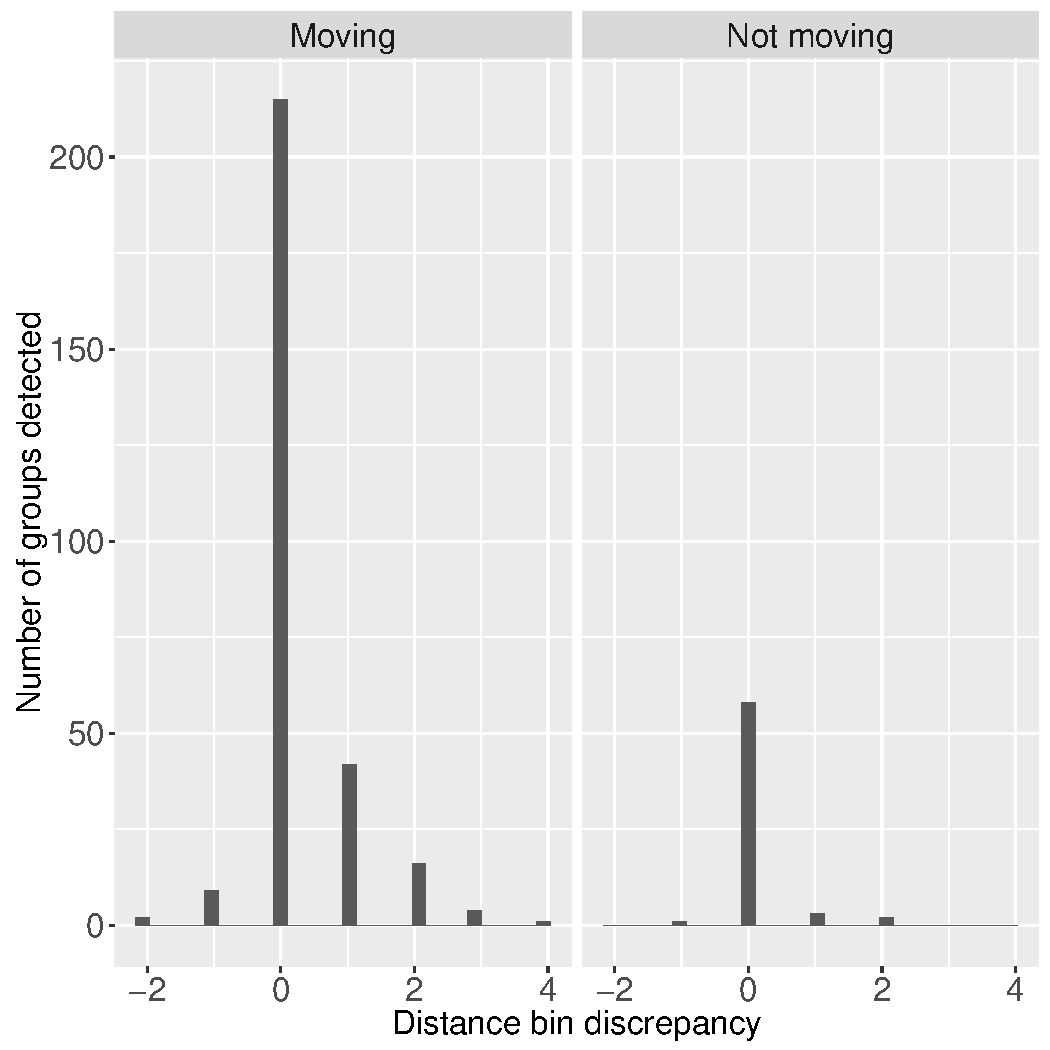
\includegraphics[width=150mm]{Dist_error_hists_JABES.pdf}
\caption{Distribution of observed distance bin discrepancies for bird groups detected by both observers in helicopter surveys. Negative values imply movement (or measurement error) towards the helicopter, while positive values imply movement away from the helicopter. For moving birds, the distance bin observed by the rear observer tended to be farther away than the bin observed by the front observer.  Since the second observer always detected birds later than the front observer, this suggests responsive movement away from the aircraft. For stationary birds, a nonzero distance bin discrepancy represents measurement error.}
\label{fig:dist_hists}
\end{center}
\end{figure*}

\pagebreak
\begin{figure*}
\begin{center}
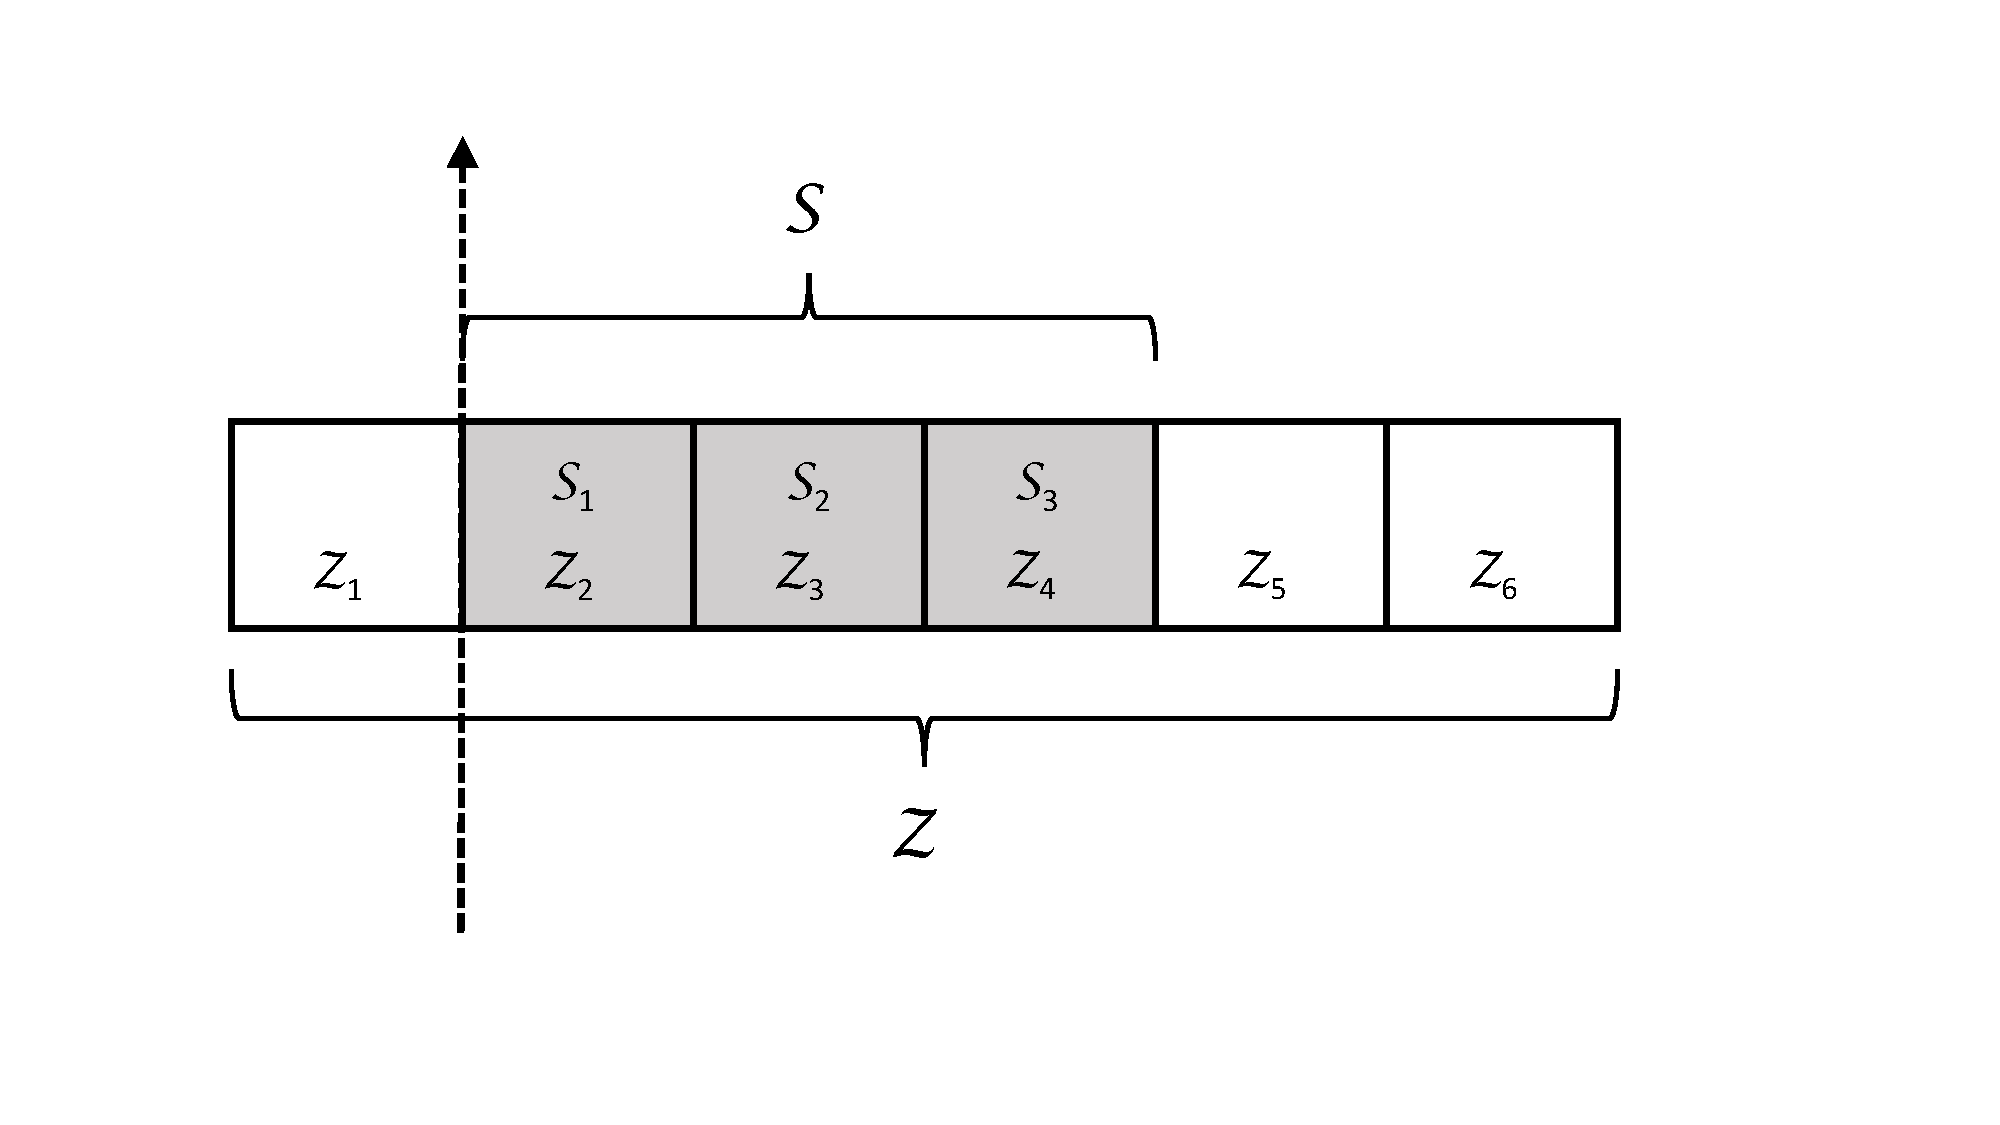
\includegraphics[width=150mm]{augmented_bin_figure.pdf}
\caption{A depiction of observed ($\mathcal{S}$) and latent ($\mathcal{Z}$) distance bins that could potentially be used in analysis of a hypothetical mark-recapture distance sampling (MRDS) survey.  In this example, only animals encountered in one of the three shaded distance bins to the right of the transect line (dashed line) are recorded; however, the state space is augmented with an additional three bins to account for possible animal movement and measurement error.  In practice, the number of augmented distance bins that are needed will be a function of the magnitude of the movement and measurement error processes.}
\label{fig:aug_bins}
\end{center}
\end{figure*}


\pagebreak
\begin{figure*}
\begin{center}
\includegraphics[width=150mm]{Kernel_plot.pdf}
\caption{Estimated movement and measurement error kernels for waterfowl mark-recapture distance sampling (MRDS) data from the highest ranked maximum marginal likelihood model. Measurement error used a (discretized) symmetric Laplace kernel, while movement had an asymmetric Laplace kernel.}
\label{fig:kernel}
\end{center}
\end{figure*}

\pagebreak
\begin{figure*}
\begin{center}
\includegraphics[width=150mm]{SpeciesN.pdf}
\caption{Estimates of bird densities and 95\% log-based confidence intervals for the surveyed region in the northern Canada from the highest ranked AIC model.  Species included Canada goose (CAGO), king eider (KIED), long-tailed duck (LTDU), northern pintail (NOPI), rock ptarmigan (ROPT), sandhill crane (SACR), and white-fronted goose (WFGO).}
\label{fig:speciesD}
\end{center}
\end{figure*}

\pagebreak
\begin{figure*}
\begin{center}
\includegraphics[width=150mm]{bootstrapGOF.pdf}
\caption{A plot of the number of observed and predicted waterfowl groups by observer and movement status.  Observed data are given by the thick solid line, while the thick dashed line represents mean predictions and the thin, dashed lines represent 2.5th and 97.5th quantiles of model-based simulations (including variance due to uncertainty of MML estimates).  }
\label{fig:GOF}
\end{center}
\end{figure*}

\pagebreak
\begin{figure*}
\begin{center}
\includegraphics[width=150mm]{DetProb_rev.pdf}
\caption{The simulated range of detection probabilities from Simulation Study 2, where heterogeneity is incorporated via a random effect on the log of the standard deviation associated with a half-normal detection model.  Solid and dashed lines represent the expected detection probability for moving and stationary animals, while shaded regions represent 95\% intervals.}
\label{fig:hn}
\end{center}
\end{figure*}

\end{document}
